\documentclass[100,a4paperpaper,]{article}

  \title{\textbf{\textcolor{white}{Relatório de Conjuntura}}}
  \author{\textbf{\textcolor{white}{Inflação}}}
  \date{\textbf{\textcolor{white}{Novembro/2021}}}
  


\newcommand{\logo}{c:/Users/700105212/R Projects/econdashboard/inst/app/www/img/logo-banestes-transparente.png}
\newcommand{\cover}{c:/Users/700105212/R Projects/econdashboard/inst/app/www/img/cover-banestes-menor.png}
\newcommand{\logotitle}{c:/Users/700105212/R Projects/econdashboard/inst/app/www/img/logo-banestes-branca.png}
\newcommand{\iblue}{004b8d}
\newcommand{\igray}{d4dbde}
\usepackage{booktabs}
\usepackage{longtable}
\usepackage{array}
\usepackage{multirow}
\usepackage{wrapfig}
\usepackage{float}
\usepackage{colortbl}
\usepackage{pdflscape}
\usepackage{tabu}
\usepackage{threeparttable}
\usepackage{threeparttablex}
\usepackage[normalem]{ulem}
\usepackage{makecell}
\usepackage{xcolor}

% Author: Karol KozioL
% License: GPL-3
% Modified by: Sarah Wagner

% % % packages -----------------------------------------------------------------------------------
\usepackage{amsmath}
\usepackage{array}
\usepackage{booktabs}
\usepackage{calc}
\usepackage{eso-pic}
\usepackage[left = 30pt, right = 30pt, top = 25pt, bottom = 25pt, headsep = 40pt, includeheadfoot]{geometry}
\usepackage{fancyhdr}
\usepackage{fontspec}
\usepackage{graphicx}
\usepackage[utf8]{inputenc}
\usepackage{lastpage}
\usepackage{multirow}
\usepackage{tabularx} 
\usepackage{tikz}
\usepackage{titlesec}
\usepackage{titling}
\usepackage{xcolor, colortbl}
\usepackage{etoolbox}
\usepackage{ragged2e}
\usepackage{xcolor}
\usepackage[fontsize=14]{scrextend}
\usepackage[portuguese]{babel}
\usepackage{indentfirst}

% % % settings -----------------------------------------------------------------------------------

% % custom colors
\definecolor{iblue}{HTML}{\iblue}
\definecolor{igray}{HTML}{\igray}

% definition of pagename
\newcommand\pagename{Page}

% % fonts 
\defaultfontfeatures{Mapping = tex-text}
\setmainfont{Arial}
\newfontfamily\headingfont{Arial}



% % sections
\titleformat{\section}{\color{iblue}\headingfont\Large\bfseries}{\thesection}{1em}{}[\titlerule]
\titleformat{\subsection}{\color{iblue}\headingfont\large\bfseries}{\thesubsection}{1em}{}
\titleformat{\subsubsection}{\color{iblue}\headingfont\large\bfseries}{\thesubsubsection}{1em}{}

% % misc
\setlength{\parindent}{0em} 
\setlength{\parskip}{1em}
\linespread{1.15}
\renewcommand{\baselinestretch}{1.25}
\raggedright
\newcolumntype{C}{>{\centering\arraybackslash}X}
\justifying


% % % custom titlepage ----------------------------------------------------------------------------
\newcommand\BackgroundPic{%
	\put(0,0){%
		\parbox[b][\paperheight]{\paperwidth}{%
			\vfill
			\centering
			
\includegraphics[width=\paperwidth,height=\paperheight]{\cover}%
			\vfill
}}}

\makeatletter

% pagestyle titlepage
\fancypagestyle{customtitle}{
	\lhead{}
	\chead{}
	\rhead{\includegraphics{\logotitle}}
	\makeatother
	\lfoot{}
	\cfoot{}
	\rfoot{}
}


% titlepage
\renewcommand{\maketitle}{
	\thispagestyle{customtitle}
	\AddToShipoutPicture*{\BackgroundPic}
	\ClearShipoutPicture
	
	\phantom{a}\hfill
	\vspace{12cm}
	
	\begin{tabular}[l]{@{}p{\textwidth}@{}}
		\color{iblue}\headingfont\LARGE\@title\\[1em]
		\color{iblue}\headingfont\Large\@author\\[1em]
		\color{iblue}\headingfont\large\@date\\[1em]
	\end{tabular}
	
	
	\clearpage
}

\makeatother

% % % header and footer ---------------------------------------------------------------------------
\pagestyle{fancy}
\lhead{}
\chead{}
\rhead{ 
\includegraphics{\logo}}
\makeatother
\newlength{\myheight}
\lfoot{}
\cfoot{}
\rfoot{\pagename~\thepage \hspace{1pt} / \pageref{LastPage}}
\renewcommand\headrulewidth{0pt}
\renewcommand\footrulewidth{0pt}




\begin{document}


\renewcommand{\contentsname}{Sumário}


\maketitle
\tableofcontents
\clearpage

\section{IPCA} 
 \vspace{0,5cm}

O Índice Nacional de Preços ao Consumidor Amplo registrou alta de 0,95\%
em novembro e 9,26\% no acumulado do ano, valor bem distante de 3,75\%
que é o centro da meta estipulada pelo Conselho Monetário Nacional
(CMN), mesmo com faixa de tolerência de 1,5 p.p para mais ou para menos.

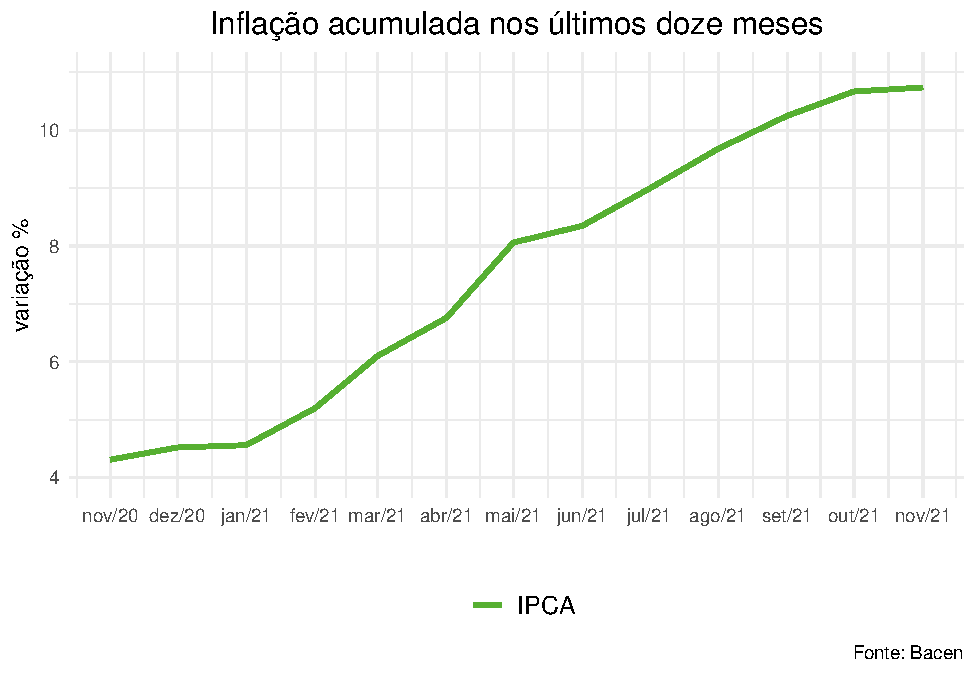
\includegraphics{inflacao_files/figure-latex/inflacao 12 meses-1.pdf}

O destaque se dá para o setor de transportes, que teve o maior aumento
do índice por três meses consecutivos. Essa variação foi influenciada
principalmente pelo preço dos combustíveis, que no acumulado do ano
sofreu aumento de 50,43\%, como a economia de modo geral depende dos
transportes esse aumento impacta diretamente todos os outros setores.
\newpage

\subsection{Combustíveis} 
 \vspace{0,5cm}

A variação no preço dos combustíveis é causada por vários fatores, um
deles foi o avanço da vacinação contra a covid-19 a nível mundial que
proporcionou a retomada global da economia, gerando uma grande demanda
por petróleo que não foi acompanhado da oferta, uma vez que no ano
passado a Organização dos Países Produtores de Petróleo (Opep) decidiu
diminuir a produção para evitar uma queda mais acentuada no nível do
preço. Com a recuperação da economia, a oferta de petróleo vem se
normalizando gradativamente enquanto a demanda cresce de forma mais
acelerada, pressionando o preço do barril.

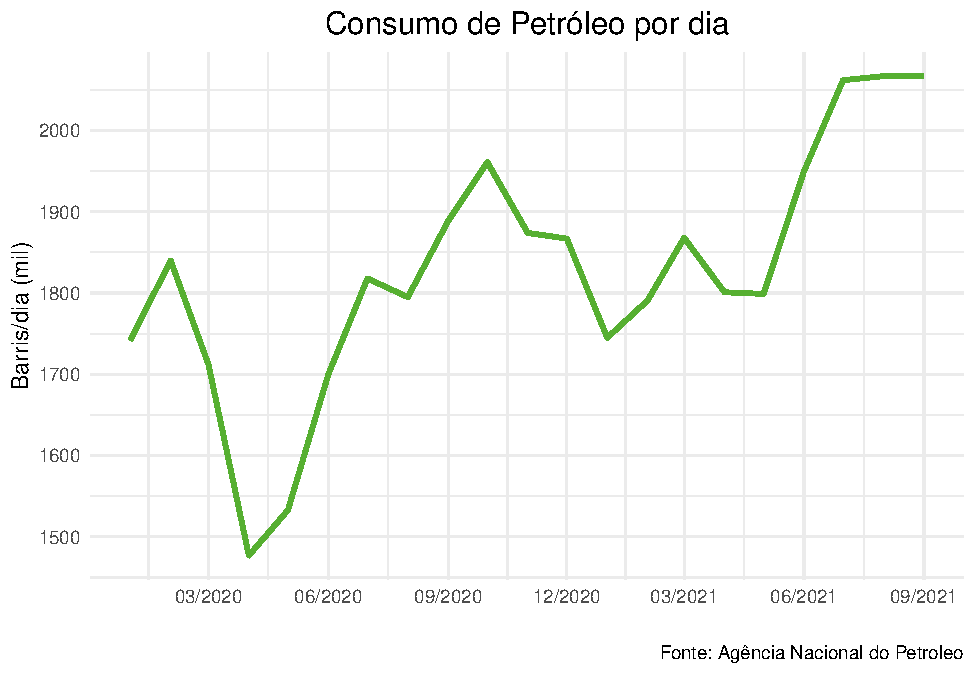
\includegraphics{inflacao_files/figure-latex/Consumo Petroleo-1.pdf}
\newpage

\subsection{Desvalorização Cambial} 
 \vspace{0,5cm}

O impacto do cenário internacional é ainda maior no Brasil devido à
desvalorização cambial, que ocorre principalmente em razão dos riscos
fiscais domésticos: especificamente a Dívida Bruta do Governo Geral
(DBGG), que compreende o governo federal, o INSS e os governos estaduais
e municipais. A DBGG atingiu 82,9\% do PIB (R\$ 7 trilhões) em outubro.
A confiança dos investidores internacionais se reduz em meio a esse
cenário, e a incerteza fiscal afasta o investimento estrangeiro.

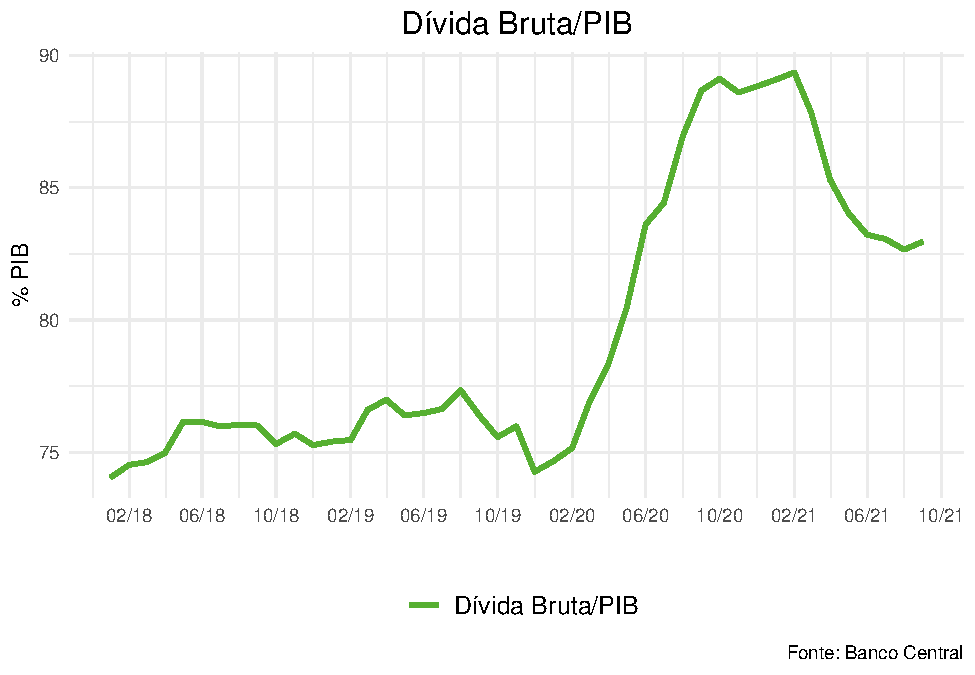
\includegraphics{inflacao_files/figure-latex/Divida Bruta/PIB-1.pdf}
\newpage

\section{Grande Vitória} 
\vspace{0,25cm}

A Grande Vitória ocupa o segundo lugar no ranking das capitais com maior
índice de inflação, com alta de 9,58\% no acumulado do ano, ficando
atrás apenas de Curitiba que teve variação de 10,97\%. Em relação à
variação mensal, a capital atingiu 1,53\% em outubro, ocupando o
primeiro lugar do ranking entre as capitais.

Um dos principais fatores que explicam essa alta inflação na região é a
habitação\footnote{O grupo habitação é composto por combustíveis domésticos
 (gás de cozinha), artigos de limpeza, energia elétrica residencial, reparos, aluguel e taxas},
que no acumulado do ano obteve a segunda maior alta do Brasil (+15\%).
Apenas em outubro, teve variação de +3,04\%, sendo o item com maior alta
da Grande Vitória, impulsionado principalmente pelo gás de botija, que
subiu 5,41\% em relação ao mês anterior.

Em relação aos alimentos e bebidas, a Grande Vitória obteve a maior alta
do país, com aumento de 2,48\% em relação ao mês anterior e variação de
7,43\% no acumulado do ano. De acordo com Departamento Intersindical de
Estatística e Estudos Socioeconômicoso (DIEESE), o custo da cesta básica
em Vitória no mês de setembro foi de R\$633,03, máxima histórica da
série desde sua criação em 1998.

\begin{center}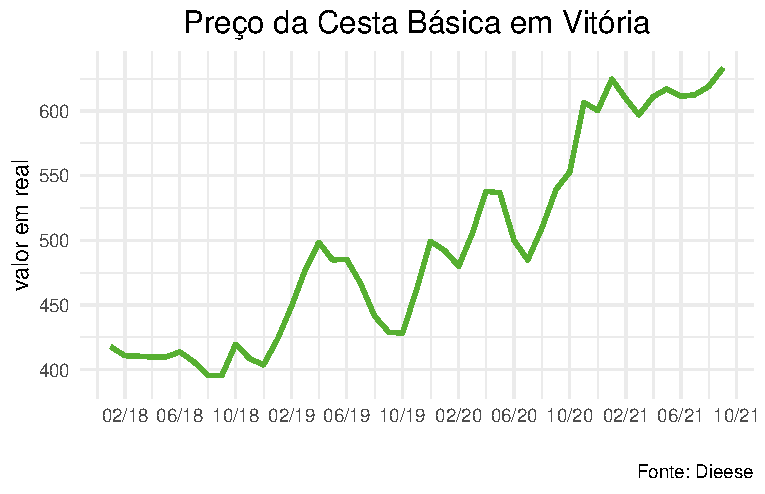
\includegraphics{inflacao_files/figure-latex/IPCA es-1} \end{center}


\end{document}
